\documentclass[main.tex]{subfiles}

\begin{document}

\section{Description of the simulation}

Modify the simulation done in assignment 1 to include Periodic Boundary Conditions. Remember that for this to work, you will need to add a cutoff to your interaction function. 

\subsection{Periodic Boundary condition}

The idea of periodic boundary conditions is to use a limited number of atoms due to computational constrains, with the intention of imitating a wider system.
This type of boundary condition treats a the simulation box like a tillable pattern, creating finite copies surrounding the original box, creating "ghost particles".
The advantage to create finite copies is that is not necessary to compute the trajectories of the ghost particles, but just the interaction between "ghost" and "real" particles.

In the following sections is a discussion to set a cut distance in the potential that helps to reduce the computational requirements, then a brief explanation on the implementation of the periodic boundary conditions and finally the results.

% We would expect the same average of properties.

\subsubsection{Cut off distance}

The first issue to analyses at consider periodic boundary conditions is the interaction between the real and ghost particles.
Adding a huge amount of ghost particles will help to improve the accuracy of the simulation, however it would cost time and computational capacity, therefore, a strategy to tackle this issue is to cut the range of the potential.

To set the cut off distance we equal the Lennard-Jones potential to a constant, $\eta$, and resolve for the distance.
To do that, the following change of variable is introduce, $\gamma = \sigma^{6}/r^{6}$, hence,
\begin{gather*}
    4\epsilon\qty(\gamma^{2} - \gamma) = \eta,
\end{gather*}
solving for $\gamma$, we get,
\begin{align*}
    \gamma &= \frac{\epsilon\pm\sqrt{\epsilon^{2}+\epsilon\eta}}{2\epsilon}, \\
    \frac{\sigma^{6}}{r^{6}} &= \frac{\epsilon\pm\sqrt{\epsilon^{2}+\epsilon\eta}}{2\epsilon},
\end{align*}
introducing a new change of variable, the expression can be written as,
\begin{gather*}
    r^{6} = \frac{\sigma^{6}}{\alpha},\qquad\alpha = \frac{\epsilon\pm\sqrt{\epsilon^{2}+\epsilon\eta}}{2\epsilon}.
\end{gather*}

Knowing that this polynomial has 6 roots, 4 of them are in the complex plane and 2 in the real set of numbers, we select the real positive root, because it has physical interpretation, since we need a positive distance of cut off,
\begin{gather*}
    r = \frac{\sigma}{\alpha^{1/6}}.
\end{gather*}
Substituting the change of variable and a recommendation of terms,
\begin{gather}
    r_{cut} = \sigma \frac{\sqrt[6]{2\epsilon}}{\sqrt[6]{\epsilon\pm\sqrt{\epsilon\qty(\epsilon+\eta)}}}. \label{eqn:rCut}
\end{gather}

To prove that the result makes physical sense, we can set $\eta = 0$, expecting to get $\sigma$ as the root of the function,
\begin{align*}
    r_{cut} &= \sigma \frac{\sqrt[6]{2\epsilon}}{\sqrt[6]{\epsilon\pm\sqrt{\epsilon\qty(\epsilon)}}}, \\
      &= \sigma \frac{\sqrt[6]{2\epsilon}}{\sqrt[6]{\epsilon\pm\epsilon}},
\end{align*}
in these case, we consider the positive root, hence
\begin{align*}
    r_{cut} &= \sigma\frac{\sqrt[6]{2\epsilon}}{\sqrt[6]{2\epsilon}}, \\
    r_{cut} &= \sigma.
\end{align*}
Therefore, we can associate the positive root near to $\sigma$, and the negative root with the largest root of the polynomial.

An interesting approach to defining $\eta$ is $\eta = \alpha\epsilon,\alpha\qty[-1,0]$.
This definition helps to define the distance of cut off in terms of the energy of the particles and equation \ref{eqn:rCut} simplifies to,
\begin{gather}
    r_{cut} = \sigma\frac{\sqrt[6]{2}}{\sqrt[6]{1\pm\sqrt{1+\alpha}}}\label{eqn:rCutf},
\end{gather}
when $\alpha=0$, then $r=\sigma$ and when $\alpha=-1$, then $r=\sqrt[6]{2}\sigma$.

In figure \ref{fig:LJpotRcutoff} we can see when $\alpha = 0,\alpha=-0.5,\alpha=-1$ .
\begin{figure}[ht]
    \centering
    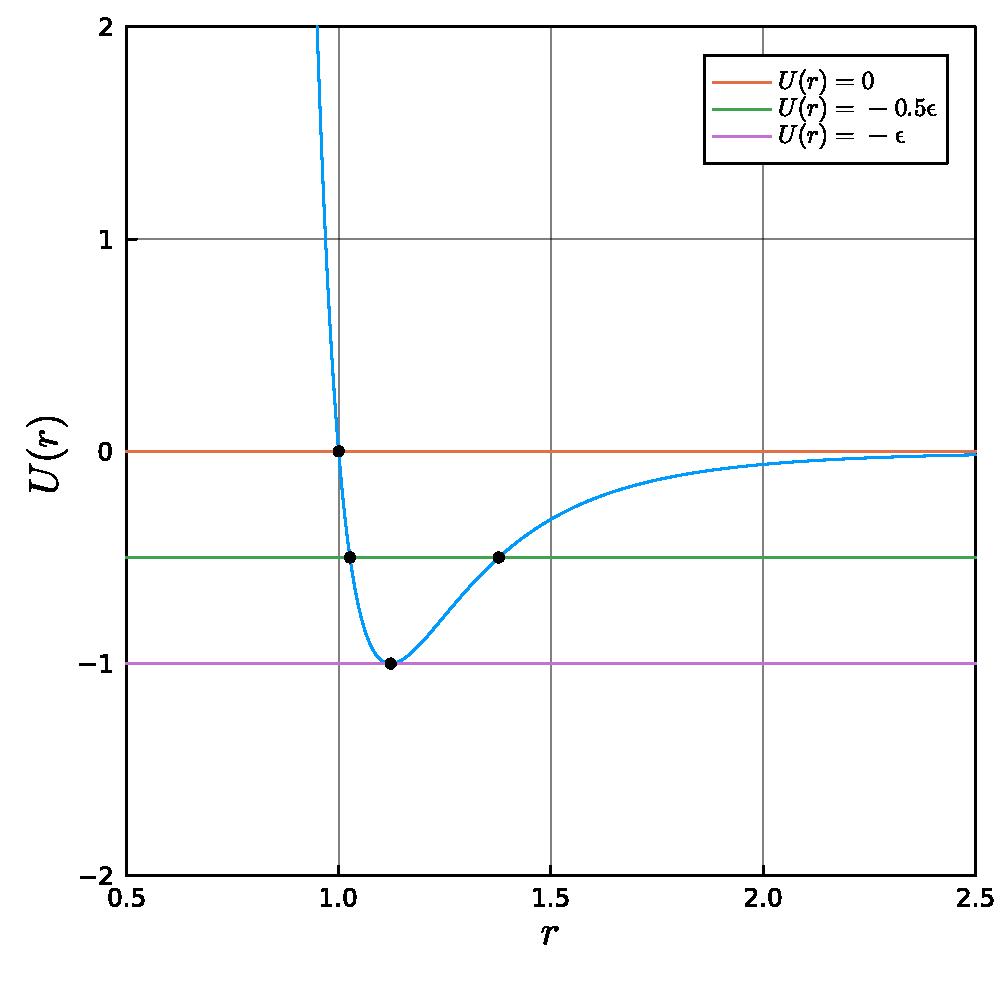
\includegraphics[width=0.7\textwidth]{imgs/hw2/LennarJonesDifferentEnergies.pdf}
    \caption{Lennard-Jones potential with intersection at energy equals to $0$,$1/2\epsilon$ and $-\epsilon$.}
    \label{fig:LJpotRcutoff}
\end{figure}

Finally, to give a physical meaning to $\eta=\alpha\epsilon$, we can relate the parameter $\epsilon$ with temperature using the equipartition theorem,
\begin{gather}
    \epsilon = \frac{3}{2}k_{B}T.
\end{gather}
At relating the temperature with the energy of the particles, we are relating the average kinetic of the system with the potential energy between particles.
It is important to notice that in equation \ref{eqn:rCut}, $\eta\in\qty[0,\epsilon]$, leading to have a system in which the potential energy between the particles needs to be greater than the average of the kinetic energy of the system, as shown in figure \ref{fig:LJpotRcutoff}.

\subsection{Implementation}

To implement the cutoff in the system, it is needed to modify the potential to avoid a discontinuity at the cut off distance.
For that, in the book \cite{libroClase} shows the expression to avoid discontinuity in the potential and the force,
\begin{gather}
    U_{rcut}\qty(r) = U_{LJ}\qty(r)-\qty(r-r_{cut})\dv{r}U\qty(r_{cut}) - U\qty(r_{cut}) \label{eqn:LJpotrcut}.
\end{gather}
In figure \ref{fig:comparisonPotantials} it shows the comparison of the Lennard-Jones potential with the potential with cutoff \ref{eqn:LJpotrcut}.
In which both potentials achieve the same minimum point, preserving the energy of the particle, however, the cut off potential decays to $0$ faster than the Lennard-Jones potential, getting the desire behavior.
%and in the figure ... is a comparison between the the force with and without the cutoff.

\begin{figure}[ht]
    \centering
    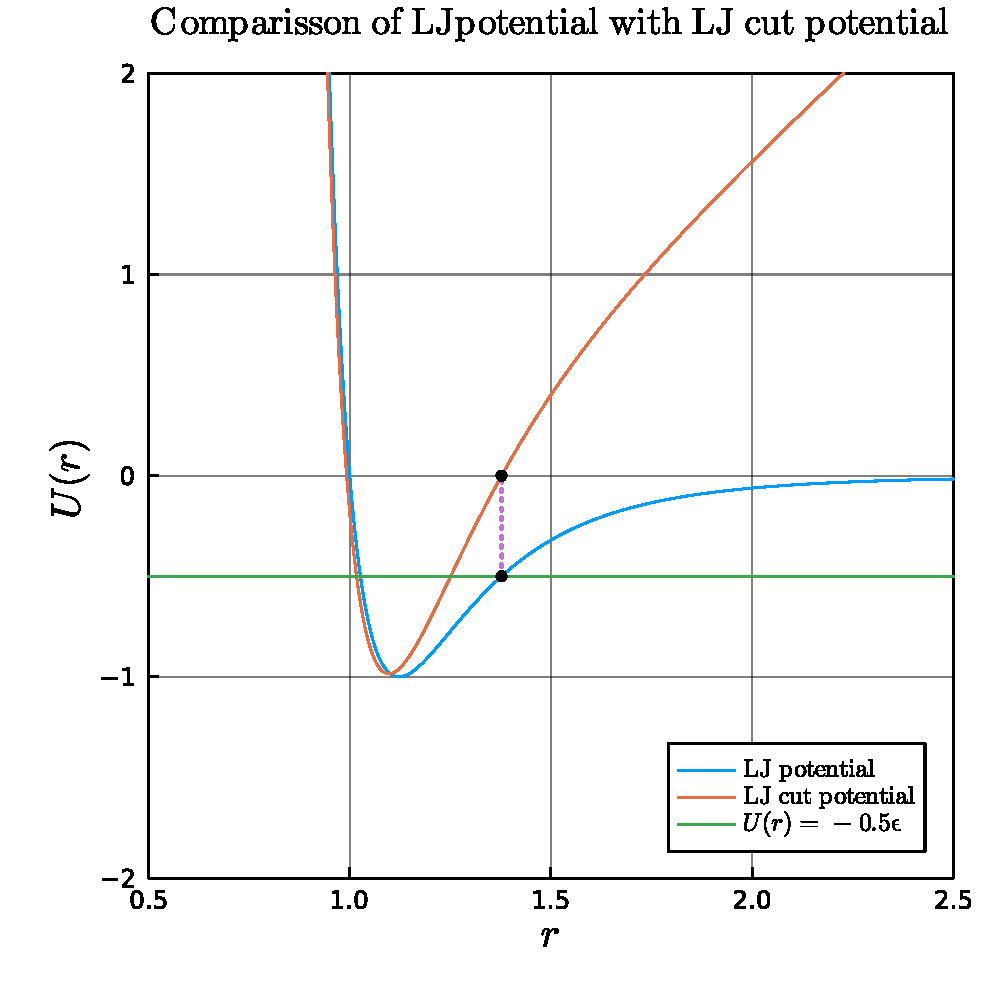
\includegraphics[width=0.7\textwidth]{imgs/hw2/LennarJonesComparison.pdf}
    \caption{Comparison between the Lennard-Jones potential with the cut off Lennard-Jones potential.
        The cut off energy is obtain with equation \eqref{eqn:rCutf} and $\alpha = -0.5$.
    }
    \label{fig:comparisonPotantials}
\end{figure}

On the other hand, the quantity of copies for the boundary conditions can be set in relation with the $r_{cut}$.
Taking into account equation \eqref{eqn:rCutf} and setting $\alpha = -0.001$, the value for $r_{cut} = 3.98405$ and the size of the box are $20\sigma$, with just one copy of the system in every direction is sufficient to use the periodic boundary condition.
In figure \ref{fig:ghostParticles} is an example of the initial condition with the ghost particles.

\begin{figure}[ht]
    \centering
    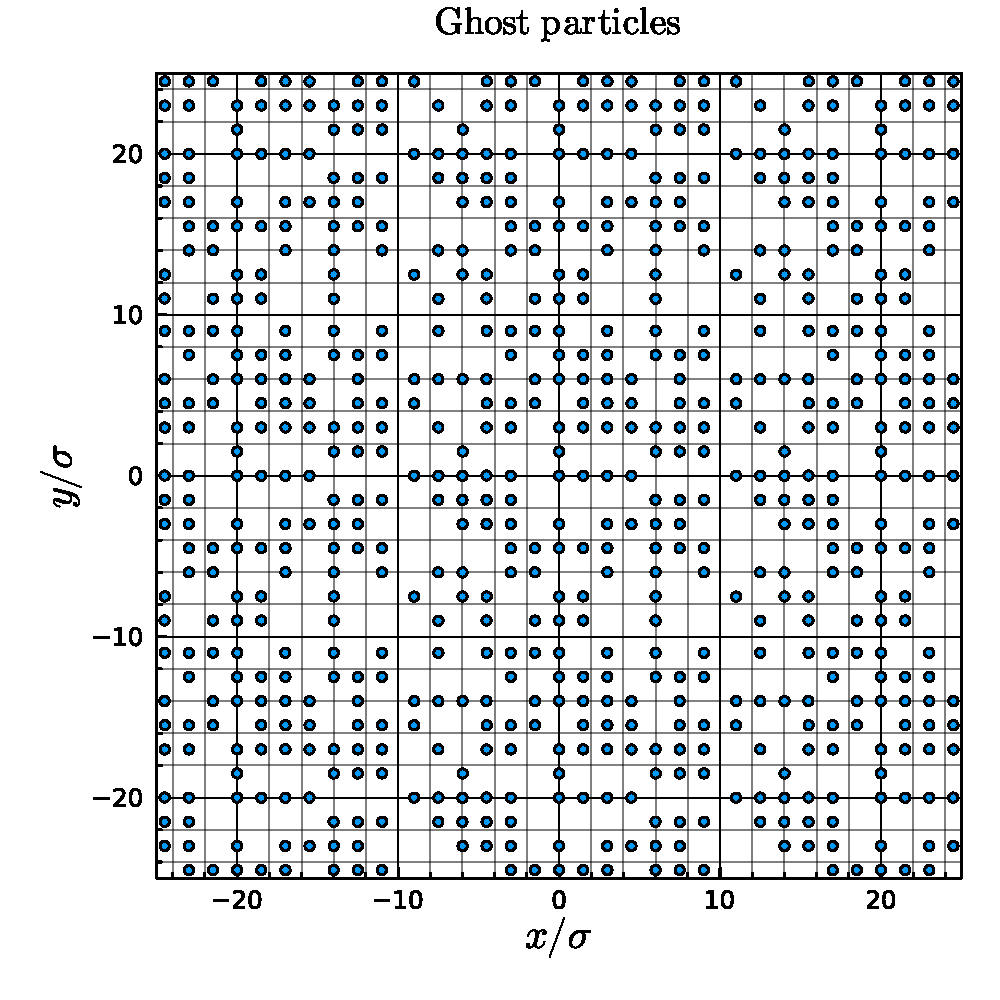
\includegraphics[width=0.7\textwidth]{imgs/hw2/ghostParticles.pdf}
    \caption{Initial condition with ghost particles. }
    \label{fig:ghostParticles}
\end{figure}

\section{Results}

Finally in figure \ref{fig:temperature} is shown the evolution of the temperature in a simulation with 100 particles in a box of $20\sigma$ by $20\sigma$ and a numerical value of $1$ for the temperature and $5$ for $\epsilon$.
It can be observed a stabilization above \num{3.8}.
The access to the animation is thru the following link \href{https://tecmx-my.sharepoint.com/:i:/g/personal/a00827546_tec_mx/EZXD87BSJGRDgFDDatIbGIgBjRzCqsQQtKEvOHwzOpqipg?email=leogabac%40tec.mx&e=McEIBo}{\color{blue}{Access to the animation}}.

\begin{figure}[ht]
    \centering
    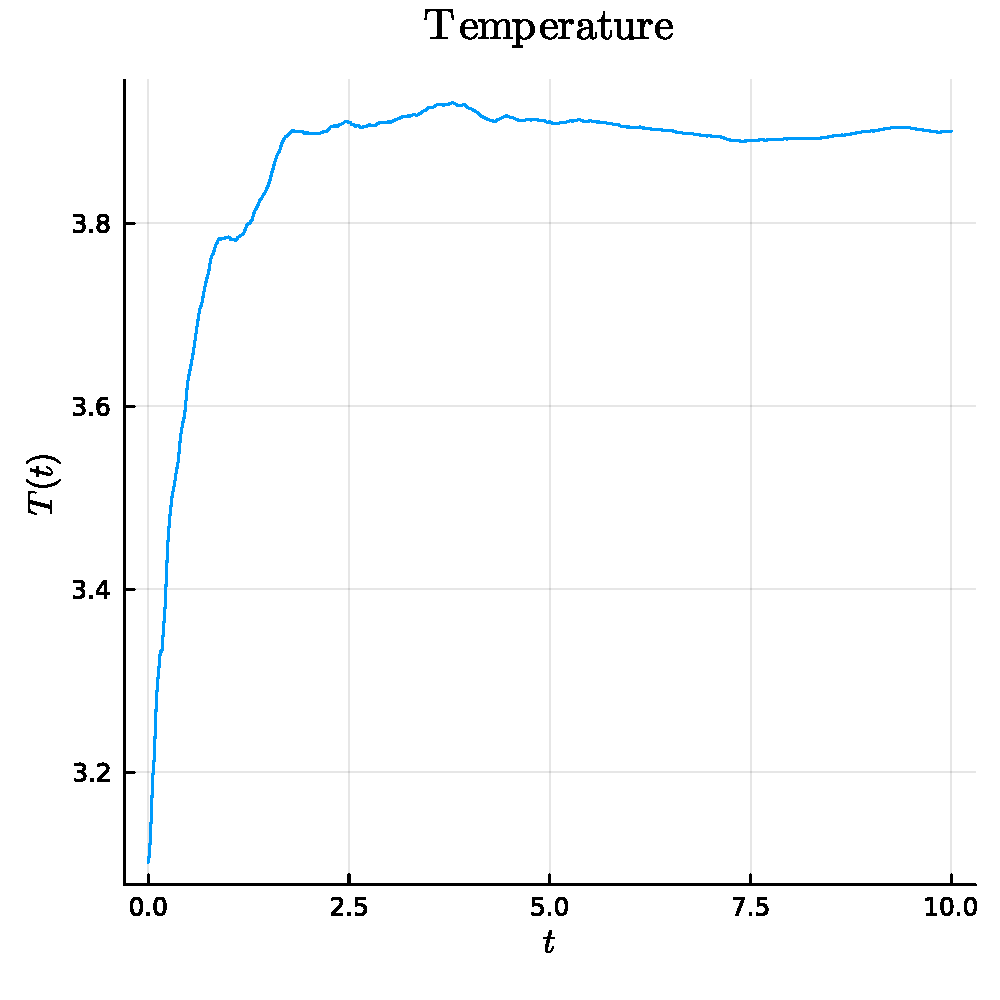
\includegraphics[width=0.7\textwidth]{imgs/hw2/100TempPlotPBC3.pdf}
    \caption{Temperature of a simulation of 100 particles in abox with periodic boundary conditions.}
    \label{fig:temperature}
\end{figure}


\begin{comment}
    

\newpage


Try to mimic something larger.

If we are in equilibrium, the density of particles remain constant.

We create a copy in the boundaries.

It is important that the rest of copies, remain as a copy of the zone of interest.
Therefore, is call as ghost particles.

We do not compute the trajectories of the ghost particles, but we do calculate the interaction with all the particles.

We would expect the same average of properties.

For long repulsion force, we can increment the quantity of copies, kwnon as Ewald summation, uses Fuorier space to reduce computational cost.

We need to difine the cutoff distance.
which is define by the energy at a certain temperature.

and we that distance, we can define the quantity of copies.

\begin{gather}
    F_{PBC} = \sum_{\vec{n}} F\qty(\vec{r}_{i,j}) + \sum_{\mu}L_{\mu}n_{\mu})
\end{gather}

$\mu$ is a direction, $n$ is the number of copies adn $L$ is the size of the space.

If $r_{cut} \leq L/2$, then $$ F(r_{ij}) = F(\mathrm{min}(r_{ij}-m_{\mu}L_{\mu})), n\in\qty[-1,0,1] $$

The increase in temperature is due to initial conditions.


The only stuff is to use a consta to make a

\begin{gather}
    4\epsilon\qty[\qty(\frac{\sigma}{r})^12 - \qty(\frac{\sigma}{r})^6] + r_{cut}
\end{gather}

If, we can cut 
\begin{gather}
    F\to r^{\gamma}, \\
    \gamma \approx = 2
\end{gather}


\begin{align*}
    \mathrm{LJp}\qty(r) &= 4\epsilon\qty[\qty(\frac{\sigma}{r})^{12} - \qty(\frac{\sigma}{r})^{6}], \\
    &= 4\epsilon \qty[\eta^{2} - \eta],\qquad \eta = \qty(\frac{\sigma}{r})^{6}, \\
    \frac{k_{B}T}{4\epsilon} &= \eta^{2} - \eta, \\
    \eta^{2} - \eta - \chi &= 0,\qquad \chi = \frac{k_{B}T}{4\epsilon}, \\
    \eta &= \frac{1 \pm\sqrt{-1^{2} + 4\chi}}{2}, \\
    \eta &= \frac{1 \pm\sqrt{1 + 4\chi}}{2}, \\
    \frac{\sigma^{6}}{r^{6}}&= \frac{1+\sqrt{1+4\chi}}{2}, \\
    r^{6} &= \frac{2\sigma^{6}}{1+\sqrt{1+4\chi}}, \\
    r &= \sqrt[6]{\frac{2\sigma^{6}}{1+\sqrt{1+4\frac{k_{B}T}{4\epsilon}}}}, \\
    &= \sqrt[6]{\frac{2\sigma^{6}}{1+\sqrt{1+\frac{k_{B}T}{\epsilon}}}}, \\
    &= \frac{2^{1/6}\sigma}{\sqrt[6]{1+\sqrt{1+\frac{k_{B}T}{\epsilon}}}}
\end{align*}

\begin{gather*}
    rcut = n length \\
    n = length/rcut
\end{gather*}

Difussion.



Title:
Numerical characterization of hydrogels for 3D printing applications.

\end{comment}


\end{document}